% The report's Figures section, written by viz/report/run_all.py from each figure script's caption; edit the
% captions in viz/report/figNN_*.py and re-run it. Each figure supports one Results paragraph, which ends with
% (Figure~\ref{...}). Needs \usepackage{graphicx} in the preamble; the PDFs are in figures/ beside this file.
% The float settings below let up to three figures share a page; they apply from here to the end of the document.
% Figures go here or at the top of a page ([!htp]), so a part-filled last page keeps its figures together at the top.
\renewcommand{\topfraction}{0.95}
\renewcommand{\bottomfraction}{0.95}
\renewcommand{\textfraction}{0.05}
\renewcommand{\floatpagefraction}{0.85}
\setcounter{topnumber}{3}
\setcounter{bottomnumber}{3}
\setcounter{totalnumber}{4}

\section{Figures}

\begin{figure}[!htp]
  \centering\small
  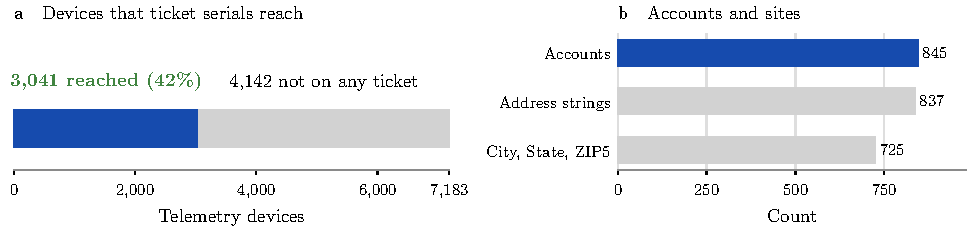
\includegraphics[width=\linewidth]{figures/fig01_ownership.pdf}
  \caption[Ticket serials and accounts]{Ticket serials reach 3,041 of 7,183 devices (42\%), and accounts are individual facilities (845 accounts at 725--837 sites), so fleets come from the installed-base list. (a)~Devices in the telemetry device table; (b)~sites counted as distinct address strings or as City, State, and ZIP5.}
  \label{fig:ownership}
\end{figure}

\begin{figure}[!htp]
  \centering\small
  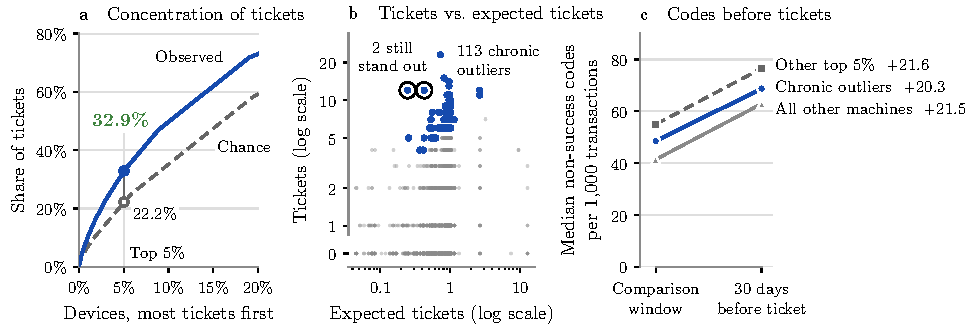
\includegraphics[width=\linewidth]{figures/fig02_high_ticket.pdf}
  \caption[High-ticket machines]{The top 5\% of the 6,621 telemetry devices hold 32.9\% of their tickets vs.~22.2\% by chance. Allowing for spread between machines, only 2 rate outliers still stand out, so high-ticket machines form a continuum. (a)~Concentration; (b)~rate outliers in blue, 2 ringed; (c)~codes rise alike.}
  \label{fig:high-ticket}
\end{figure}

\begin{figure}[!htp]
  \centering\small
  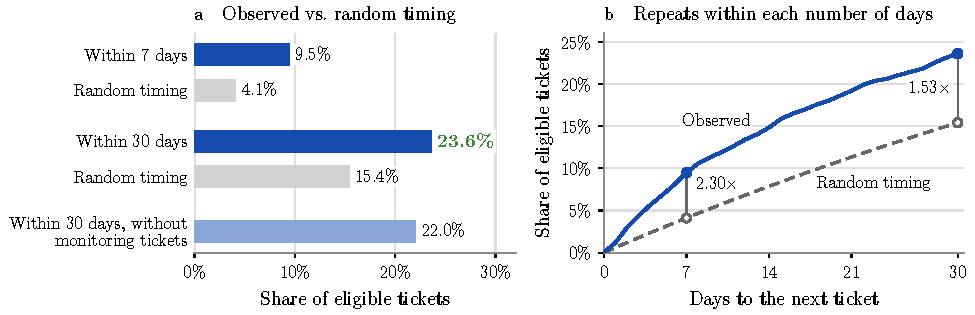
\includegraphics[width=\linewidth]{figures/fig03_repeats.pdf}
  \caption[Repeat tickets vs. random timing]{Of 6,665 eligible tickets, 23.6\% repeat within 30 days and 9.5\% within 7 days, 1.53 and 2.30 times random timing's shares, and without monitoring tickets the 30-day share is 22.0\%. (a)~Shares at 7 and 30 days; (b)~shares within each number of days up to 30.}
  \label{fig:repeats}
\end{figure}

\begin{figure}[!htp]
  \centering\small
  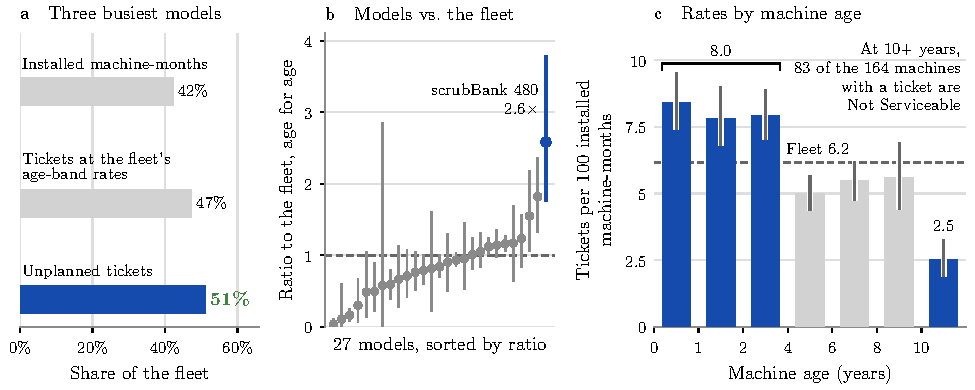
\includegraphics[width=\linewidth]{figures/fig04_rates.pdf}
  \caption[Rates by model and age]{The three busiest models hold 42\% of machine-months and 51\% of tickets, partly because they are younger; scrubBank 480 runs 2.6 times the fleet age for age; machines under 4 years run about 8 per 100 vs.~2.5 at 10 years or more. (a)~Shares; (b)~by model; (c)~by age; 95\% intervals.}
  \label{fig:rates}
\end{figure}

\begin{figure}[!htp]
  \centering\small
  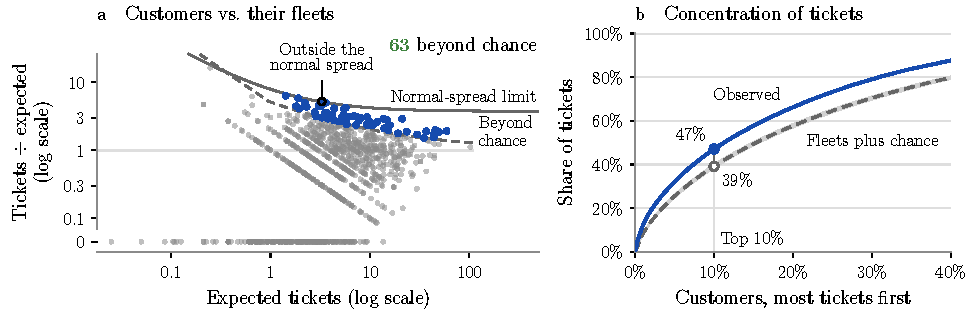
\includegraphics[width=\linewidth]{figures/fig05_customers.pdf}
  \caption[Customers vs. their fleets]{63 customers exceed their fleets beyond chance (1,732 tickets vs.~747 expected), and 1 lies outside the normal spread; the top 10\% of customers hold 47\% of tickets vs.~39\% from their fleets plus chance. (a)~1,056 customers; (b)~band, the middle 95\% of 1,000 chance draws.}
  \label{fig:customers}
\end{figure}

\begin{figure}[!htp]
  \centering\small
  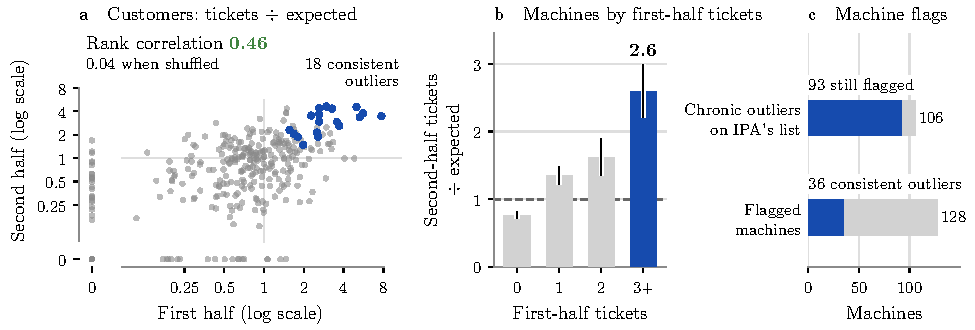
\includegraphics[width=\linewidth]{figures/fig06_persistence.pdf}
  \caption[Persistence and outliers]{Customers above their fleets in the first half tend to stay above them in the second (rank correlation 0.46 vs.~0.04 when shuffled), and machines with 3 or more first-half tickets had 2.6 times their expected second-half tickets. (a)~Customers; (b)~95\% intervals; (c)~no separate group.}
  \label{fig:persistence}
\end{figure}

\begin{figure}[!htp]
  \centering\small
  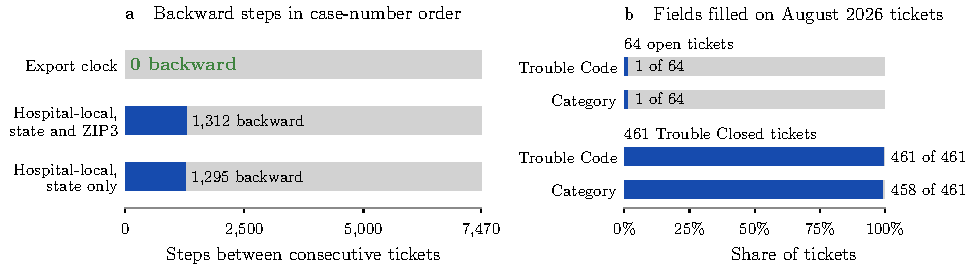
\includegraphics[width=\linewidth]{figures/fig07_clock.pdf}
  \caption[Ticket clock and issue fields]{Opening times never step backwards in case-number order (0 of 7,470 steps) but would 1,295--1,312 times on hospital-local clocks. (a)~Two zone maps; (b)~Trouble Code and Category are filled on 1 of 64 open tickets vs.~nearly all of 461 August 2026 Trouble Closed tickets of any kind.}
  \label{fig:clock}
\end{figure}

\begin{figure}[!htp]
  \centering\small
  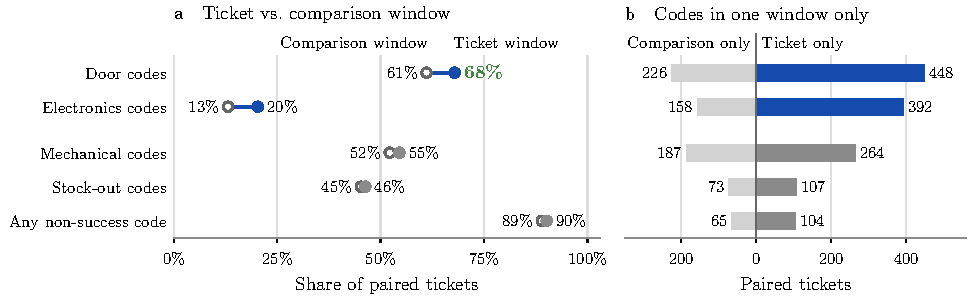
\includegraphics[width=\linewidth]{figures/fig08_first_look.pdf}
  \caption[First look at codes]{Door codes appear before 68\% of the 3,259 paired tickets vs.~61\% of their comparison windows, and electronics codes before 20\% vs.~13\%. (a)~Share with a code of the group among each window's last 10 codes; (b)~tickets with the group in one window only.}
  \label{fig:first-look}
\end{figure}

\begin{figure}[!htp]
  \centering\small
  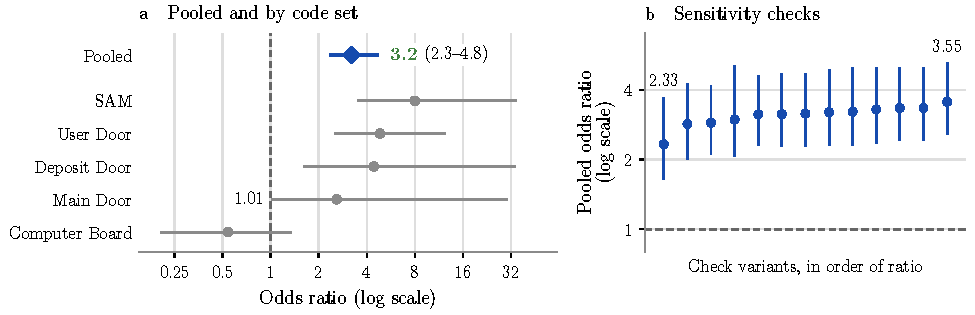
\includegraphics[width=\linewidth]{figures/fig09_association.pdf}
  \caption[Association results]{The odds that a ticket's own codes appear in its final 7 days rather than in its comparison window's are 3.2 times those of other faults' tickets (95\% interval 2.3--4.8), a provisional result resting almost entirely on scrubex machines. (a)~By code set; (b)~by check variant; 95\% intervals.}
  \label{fig:association}
\end{figure}

\begin{figure}[!htp]
  \centering\small
  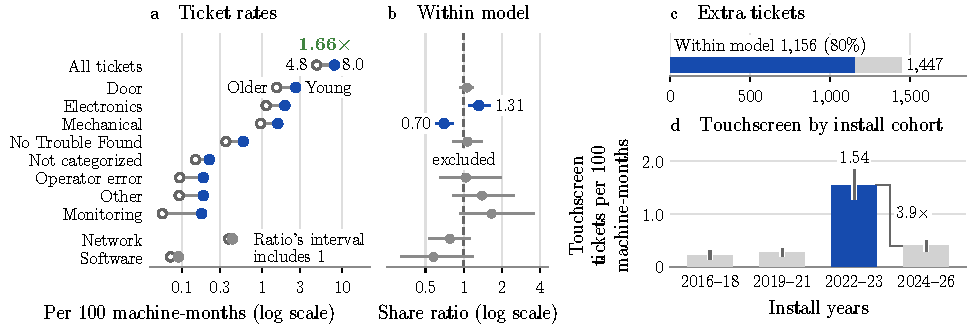
\includegraphics[width=\linewidth]{figures/fig10_request_types.pdf}
  \caption[Request types by age]{Young machines run 8.0 tickets per 100 machine-months vs.~4.8 for older ones (1.66 times), with higher rates in nearly every request group. (a)~By request group; (b)~share ratios; (c)~1,447 extra tickets, 80\% within model; (d)~Touchscreen by cohort; 95\% intervals.}
  \label{fig:request-types}
\end{figure}

\begin{figure}[!htp]
  \centering\small
  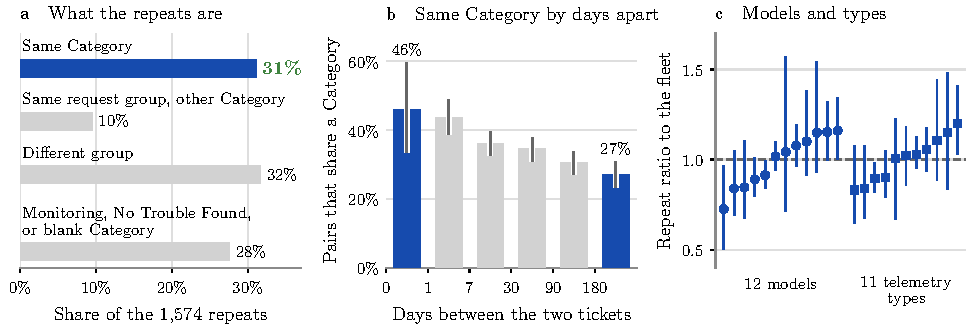
\includegraphics[width=\linewidth]{figures/fig11_pairings.pdf}
  \caption[Repeat-contact pairings]{Of the 1,574 repeats, 31\% are the same Category, and 46\% of pairs of a machine's tickets a day or less apart share a Category vs.~27\% over six months apart. (a)~By class; (b)~by gap; (c)~no model or telemetry type with 100 or more eligible tickets clearly stands out; 95\% intervals.}
  \label{fig:pairings}
\end{figure}

\begin{figure}[!htp]
  \centering\small
  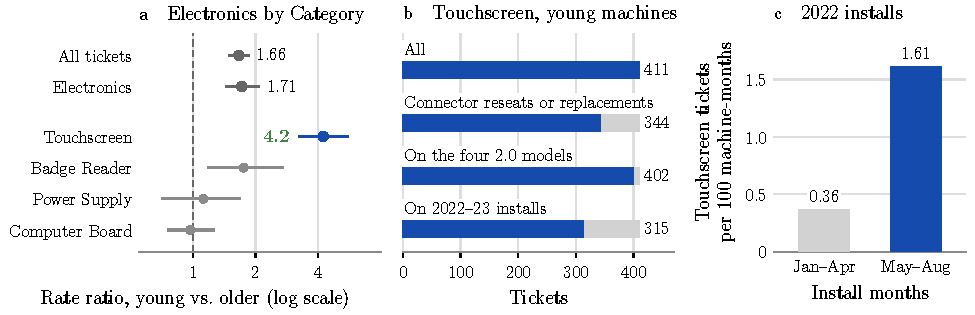
\includegraphics[width=\linewidth]{figures/fig12_electronics.pdf}
  \caption[Electronics cases]{Per machine-month, Electronics runs 1.71 times as often on young machines, near the 1.66 for all tickets, and Touchscreen stands out at 4.2 times. (a)~Categories with 30 or more tickets in each age group, 95\% intervals; (b)~its 411 young-machine tickets; (c)~from 11 and 53 tickets.}
  \label{fig:electronics}
\end{figure}

\begin{figure}[!htp]
  \centering\small
  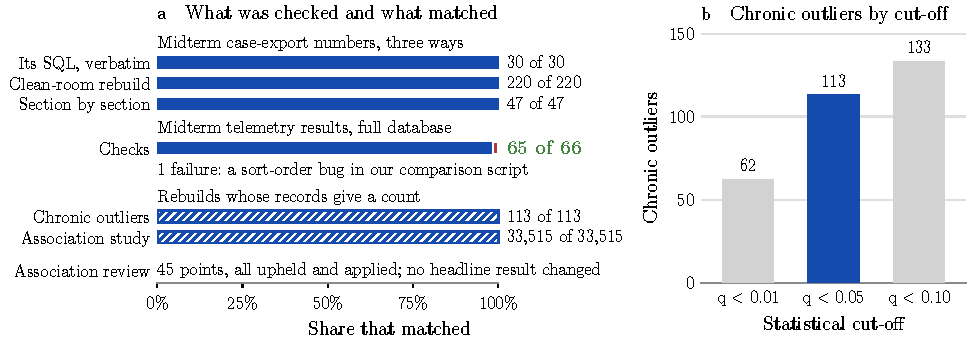
\includegraphics[width=\linewidth]{figures/fig13_verification.pdf}
  \caption[Verification]{Every case-export number reproduced exactly, and on the full database 65 of 66 checks passed; the chronic-outlier count runs from 62 to 133 with the statistical cut-off. (a)~Recounted (solid) or as recorded (hatched); (b)~among the 6,621 telemetry devices.}
  \label{fig:verification}
\end{figure}

\clearpage
